\documentclass[
	classe=$1^{ere}STI2D$
]{coursclass}

\usetikzlibrary{calc,positioning}

\renewcommand{\arraystretch}{1.4}

\title{Chapitre 7 : Lois de probabilités}
\date{}

\begin{document}

\maketitle

\begin{definition}[Arbre de probabilités]
	Une expérience aléatoire peut être représentée par un \textbf{arbre de probabilités} si elle est composée de plusieurs \textit{épreuves}.

	Deux épreuves sont \textbf{indépendantes} lorsque le résultat de l'une n'influence pas la probabilité des résultats de l'autre.
\end{definition}

\begin{exemple}
	On fait une expérience qui consiste à lancer un dé équilibré 3 fois de suite, et à regarder si on a obtenu un $6$.

	On note $A$ l'évènement «Le dé est tombé sur $6$». Ainsi on peut dessiner l'arbre suivant :
	\begin{center}
		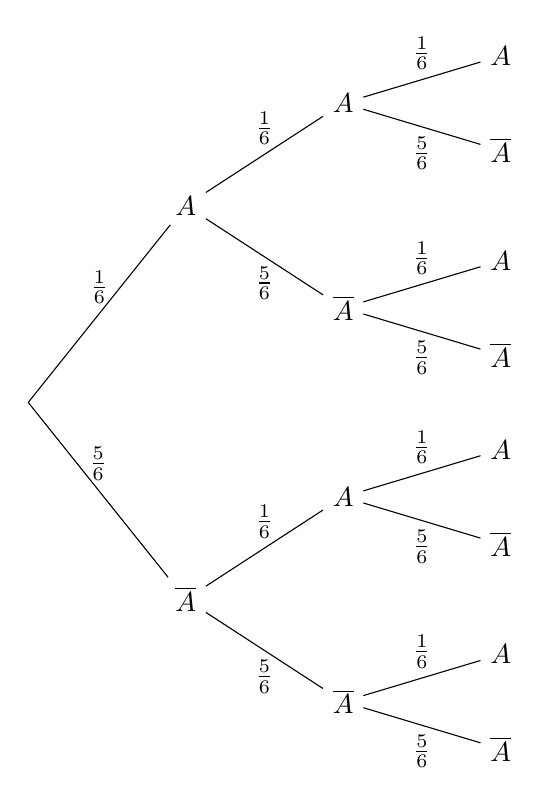
\begin{tikzpicture}
			\coordinate (START) at (0,0);
			\node (A) at (2,2.5) {$A$};
			\node (NA) at (2,-2.5) {$\overline{A}$};
			\draw (START) -- node[above] {$\frac{1}{6}$} (A)
			(START) -- node[above] {$\frac{5}{6}$} (NA);
			\foreach \n in {A,NA} {
					\node (Ab) at ($(\n) + (2,1.3)$) {$A$};
					\node (NAb) at ($(\n) + (2,-1.3)$) {$\overline{A}$};
					\draw (\n) -- node[above] {$\frac{1}{6}$} (Ab);
					\draw (\n) -- node[below] {$\frac{5}{6}$} (NAb);
					\foreach \nb in {Ab,NAb} {
							\node (Ac) at ($(\nb) + (2,0.6)$) {$A$};
							\node (NAc) at ($(\nb) + (2,-0.6)$) {$\overline{A}$};
							\draw (\nb) -- node[above] {$\frac{1}{6}$} (Ac);
							\draw (\nb) -- node[below] {$\frac{5}{6}$} (NAc);
						}
				}
		\end{tikzpicture}
	\end{center}
\end{exemple}

\begin{propriete}[Probabilité d'une issue]
	Si les épreuves que représente notre arbre sont indépendantes, la probabilité d'une issue est le \textbf{produit} des probabilités du chemin qui mène à cette issue.
\end{propriete}

\begin{exemple}
	Dans l'exemple précédent, l'issue «On a obtenu un  six \textit{uniquement} au premier lancé» est représentée par le chemin $(A, \overline{A}, \overline{A})$. Sa probabilité est alors $\dfrac{1}{6} × \dfrac{5}{6} × \dfrac{5}{6} = \dfrac{25}{216}$.
\end{exemple}

\begin{propriete}[Probabilité d'un évènement]
	La probabilité d'un évènement est la somme des probabilités des issues qui forment cet évènement.
\end{propriete}

\begin{exemple}
	Si on veut obtenir la probabilité d'obtenir \textit{exactement} $1$ six sur les trois lancés :

	Cet évènement est constitué des issues $(A, \overline{A}, \overline{A})$, $(\overline{A}, A, \overline{A})$ et $(\overline{A}, \overline{A}, A)$. Sa probabilité est donc

	\begin{center}
		\begin{tikzpicture}
			\coordinate (START) at (0,0);
			\node (A) at (2,2.5) {$A$};
			\node (NA) at (2,-2.5) {$\overline{A}$};
			\draw (START) -- node[above] {$\frac{1}{6}$} (A)
			(START) -- node[above] {$\frac{5}{6}$} (NA);
			\foreach \n in {A,NA} {
					\node (Ab) at ($(\n) + (2,1.3)$) {$A$};
					\node (NAb) at ($(\n) + (2,-1.3)$) {$\overline{A}$};
					\draw (\n) -- node[above] {$\frac{1}{6}$} (Ab);
					\draw (\n) -- node[below] {$\frac{5}{6}$} (NAb);
					\foreach \nb in {Ab,NAb} {
							\node (Ac) at ($(\nb) + (2,0.6)$) {$A$};
							\node (NAc) at ($(\nb) + (2,-0.6)$) {$\overline{A}$};
							\draw (\nb) -- node[above] {$\frac{1}{6}$} (Ac);
							\draw (\nb) -- node[below] {$\frac{5}{6}$} (NAc);
						}
				}
			\coordinate (TEMP) at (6,0.6);
			\node[right=of TEMP] {→ issue $(A, \overline{A}, \overline{A})$, probabilité $\dfrac{1}{6} × \dfrac{5}{6} × \dfrac{5}{6} = \dfrac{25}{216}$};
			\coordinate (TEMP) at (6,-1.8);
			\node[right=of TEMP] {→ issue $(\overline{A}, A, \overline{A})$, probabilité $\dfrac{5}{6} × \dfrac{1}{6} × \dfrac{5}{6} = \dfrac{25}{216}$};
			\coordinate (TEMP) at (6,-3.2);
			\node[right=of TEMP] {→ issue $(\overline{A}, \overline{A}, A)$, probabilité $\dfrac{5}{6} × \dfrac{5}{6} × \dfrac{1}{6} = \dfrac{25}{216}$};
		\end{tikzpicture}

		$$ \dfrac{25}{216} + \dfrac{25}{216} + \dfrac{25}{216} = \dfrac{75}{216} = \dfrac{25}{72} $$
	\end{center}
\end{exemple}

\begin{definition}[Variable aléatoire]
	Dans une expérience aléatoire, une \textbf{variable aléatoire} est un nombre réel associé à chaque issue de l'expérience. On la note avec une lettre majuscule, souvent (mais pas toujours !) $X$ ou $Y$.

	Ainsi on peut définir des \textit{évènements} liés à cette variable aléatoire :
	\begin{itemize}
		\item $\{X = a\}$ désigne l'évènement « $X$ prend la valeur $a$ »
		\item $\{X < a\}$ désigne l'évènement « $X$ prend une valeur strictement inférieure à $a$ »
	\end{itemize}
\end{definition}

\begin{exemple}
	On lance trois dés, et :
	\begin{itemize}
		\item Si on obtient $3$ six, on gagne $1000$€.
		\item Sinon, on perd $10$€.
	\end{itemize}
	Ici la variable aléatoire est le gain $G$ que l'on peut obtenir, en euros. Il y a deux possibilités :
	\begin{itemize}
		\item Si on fait $3$ six, alors $G = +1000$. On a donc $P(G = 1000) = \dfrac{1}{216}$ (la probabilité de faire $3$ six).
		\item Sinon, $G = -10$. On a donc $P(G = -10) = \dfrac{215}{216}$.
	\end{itemize}

	On dira que l'issue $(6 ; 6 ; 6)$ est \textbf{favorable} à l'évènement $\{G = 1000\}$, tandis que les issues $(1 ; 1 ; 1)$, $(2 ; 3 ; 2)$, etc... sont favorable à l'évènement $\{G = -10\}$.
\end{exemple}

\begin{definition}[Loi de probabilité]
	Pour une variable aléatoire $X$, sa \textbf{loi de probabilité} est la description des probabilités associées à chaque valeur possible de $X$.
\end{definition}

\begin{exemple}
	Dans l'exemple ci-dessus, la loi de probabilité de $G$ est
	\begin{itemize}
		\item $P(G = 1000) = \dfrac{1}{216}$
		\item $P(G = -10) = \dfrac{215}{216}$
	\end{itemize}

	\uline{Noter que le total des probabilités est toujours $1$.}
\end{exemple}

\begin{definition}[Espérance]
	L'\textbf{espérance} d'une variable aléatoire $X$ est la valeur de la moyenne que l'on peut \textit{espérer} obtenir si on répète l'expérience un grand nombre de fois.

	Si la loi de probabilité de $X$ est donnée par
	\begin{center}
		\begin{tabular}{|c|c|c|c|c|}
			\hline
			$a_i$        & $a_1$ & $a_2$ & $⋯$ & $a_n$ \\ \hline
			$P(X = a_i)$ & $p_1$ & $p_2$ & $⋯$ & $p_n$ \\ \hline
		\end{tabular}
	\end{center}

	Alors son espérance est
	$$ E(X) = p_1a_1 + p_2a_2 + ⋯ + p_na_n $$
\end{definition}

\begin{exemple}
	Si on jette un dé équilibré à six faces, et que l'on défini la variable aléatoire $X$ telle que :
	\begin{itemize}
		\item Si on obtient $1$, $2$, $3$ ou $4$, $X = 0$.
		\item Si on obtient $5$, $X = 1$.
		\item Si on obtient $6$, $X = 2$.
	\end{itemize}

	On a alors le tableau suivant :
	\begin{tabular}{|c|c|c|c|}
		\hline
		$a$        & $0$            & $1$            & $2$            \\ \hline
		$P(X = a)$ & $\frac{4}{6}$ & $\frac{1}{6}$ & $\frac{1}{6}$ \\ \hline
	\end{tabular}

	Et donc
	\begin{align*}
		E(X) & = \dfrac{4}{6}×0 + \dfrac{1}{6}×1 + \dfrac{1}{6}×2 \\
		     & = 0 + \dfrac{1}{6} + \dfrac{2}{6}                  \\
		     & = \dfrac{1}{2}
	\end{align*}
\end{exemple}

\end{document}